\documentclass[
]{jss}

\usepackage[utf8]{inputenc}

\providecommand{\tightlist}{%
  \setlength{\itemsep}{0pt}\setlength{\parskip}{0pt}}

\author{
FirstName LastName\\University/Company \And Second Author\\Affiliation
}
\title{A Capitalized Title: Something about a Package \pkg{foo}}

\Plainauthor{FirstName LastName, Second Author}
\Plaintitle{A Capitalized Title: Something about a Package foo}
\Shorttitle{\pkg{foo}: A Capitalized Title}

\Abstract{
The abstract of the article.
}

\Keywords{keywords, not capitalized, \proglang{Java}}
\Plainkeywords{keywords, not capitalized, Java}

%% publication information
%% \Volume{50}
%% \Issue{9}
%% \Month{June}
%% \Year{2012}
%% \Submitdate{}
%% \Acceptdate{2012-06-04}

\Address{
    FirstName LastName\\
  University/Company\\
  First line Second line\\
  E-mail: \email{name@company.com}\\
  URL: \url{http://rstudio.com}\\~\\
    }


% Pandoc header

\usepackage{amsmath}

\begin{document}

\hypertarget{net---map}{%
\subsection{Net - Map}\label{net---map}}

\begin{CodeChunk}


\begin{center}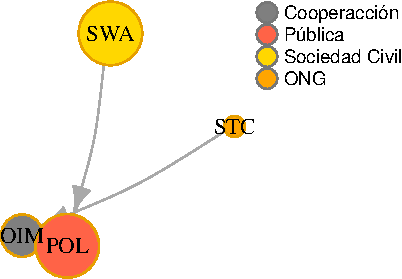
\includegraphics{netmap_oim_files/figure-latex/unnamed-chunk-2-1} \end{center}

\end{CodeChunk}

\hypertarget{asociaciones}{%
\section{Asociaciones}\label{asociaciones}}

\begin{CodeChunk}


\begin{center}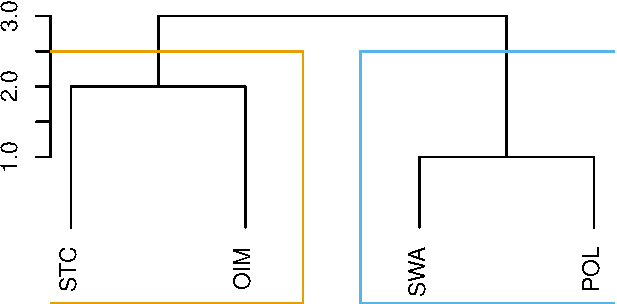
\includegraphics{netmap_oim_files/figure-latex/unnamed-chunk-3-1} \end{center}

\end{CodeChunk}

\begin{CodeChunk}


\begin{center}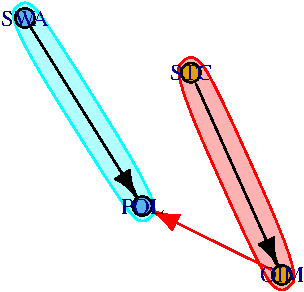
\includegraphics{netmap_oim_files/figure-latex/unnamed-chunk-4-1} \end{center}

\end{CodeChunk}



\end{document}

